\chapter{Mastodon Dataset Analysis} \label{dataset-description}

\begin{table}[tb]
    \centering\small
    \renewcommand{\arraystretch}{1.3}
    \begin{tabularx}{\textwidth}{lX}
        \toprule
        \textbf{Field} & \textbf{Description} \\
        \midrule
        \texttt{id} & Unique identifier for each toot \\
        \texttt{content} & The toot content in HTML format (converted to plain text for analysis) \\
        \texttt{crawled\_from\_instance} & The instance where the toot was observed \\
        \texttt{instance} & The home instance of the posting user \\
        \texttt{is\_local} & Boolean indicating whether the toot originated on the crawled instance \\
        \texttt{created\_at} & Timestamp of toot creation \\
        \texttt{sensitive} & Flag marking potentially sensitive content \\
        \texttt{spoiler\_text} & Content warnings or spoiler alerts \\
        \texttt{language} & Language of the posting user \\
        \bottomrule
    \end{tabularx}
    \caption{Key fields available in the Mastodon dataset with their descriptions.}
    \label{dataset-fields}
\end{table}

The dataset used in this study consists of public toots collected from a federated network of instances. The data was gathered using a distributed crawler developed by \citet{wiegmann:2024}, which collects toots from Mastodon instances' public timelines via their REST API while respecting user privacy settings. The crawler stores the collected data in an Elasticsearch cluster with careful attention to ethical considerations, never publishing raw user data.

As reported by \citet{wiegmann:2024} in November~2024, the corpus contained 733~million toots collected over 61~days from 1,015~instances. The complete dataset includes detailed metadata about each toot and relationships between instances, with key fields described in Table~\ref{dataset-fields}. Approximately 95\% of the entries were duplicates, reflecting the federated nature of Mastodon, where content is frequently shared across instances. While the crawler has continued running since the report by \cite{wiegmann:2024}, our analysis focuses specifically on English-language toots from the complete year~2024, collected from 1,000~fully crawled instances.

Approximately 18\% of toots contain media attachments (mostly images). Because our toxicity detection models analyze only text content, we removed those with media attachments. In addition, we filter out reblogs (boosts) because they do not contain original content in our dataset---instead, only the ID and URL of the boosted toot are stored, while the actual content must be fetched separately. The final dataset contains around 1.8~billion toots.

For our analysis, we use a~1\% subsample of 17,691,031 toots. This approach was chosen due to insufficient time to process the entire dataset and the challenges associated with handling such a large volume of data. The subset is generated by randomly selecting 10 toots from each batch of 1000 in parallel during the preprocessing step of our pipeline. The batches cover short, continuous time spans, preserving the temporal structure of the dataset. 

\newpage
After subsampling, the subset exhibits the following key characteristics:

\begin{itemize}
\item Approximately 20\% originate from "mastodon.social" posted aross instances.
\item While the origin of the toots is heavily centered on one instance, the distribution of the instances where the toots were posted is more balanced (see Figure~\ref{instance-distribution}).
\item During subsampling, 71 weakly represented instances were removed, leaving 929 instances.
\item The proportion of duplicates is reduced to 50\% (from 95\% in the original dataset).
\end{itemize}

\begin{figure}[tb]
    \centering
    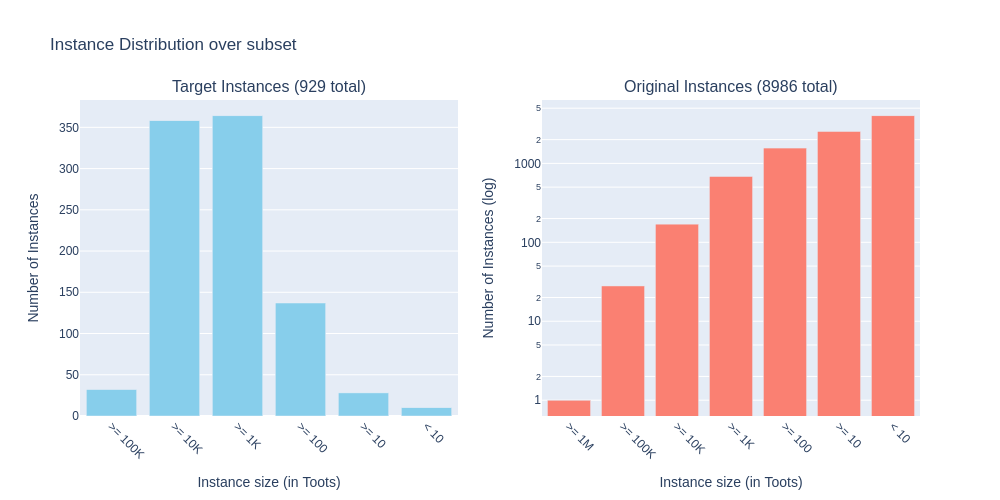
\includegraphics[width=\textwidth]{../material/instance_distribution.png}
    \caption{Distribution of Toot Counts per Instance: Comparison of Sources vs. Targets. The left chart shows the number of instances by toot volume for the target instances, while the right chart (log scale) shows the same for the source instances.}
    \label{instance-distribution}
\end{figure}

As shown in Figure~\ref{toot-distribution}, the subsample maintains consistent temporal coverage throughout 2024. October and November saw an increase in the number of toots posted. This can be explained by the election campaign and the elections in the USA. There is also an extreme peak in toots marked as sensitive on the 6th of November 2024 (Figure~\ref{sensitive-toots}). As this was the first day after the U.S. election, the observed trends may reflect heightened toxicity related to Donald Trump’s electoral outcome. As \citet{he:2023} already described, mastodon.social dominates as users' home instance due to its size.

\begin{figure}[tb]
    \centering
    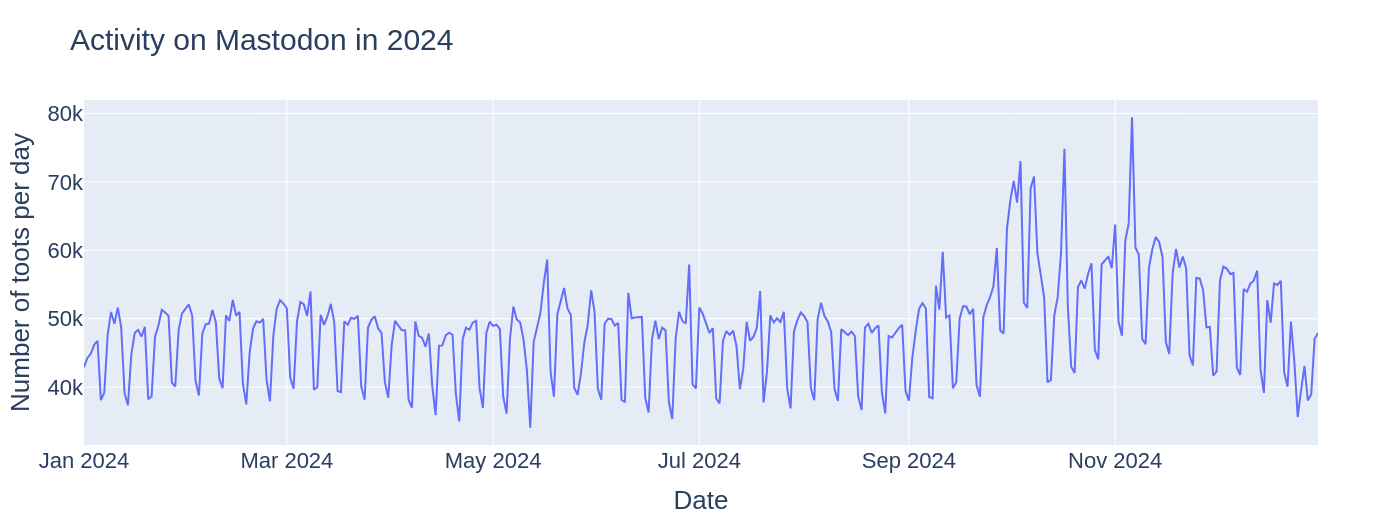
\includegraphics[width=\textwidth]{../material/activity_2024.png}
    \caption{Total number of toots in our subset per day.}
    \label{toot-distribution}
    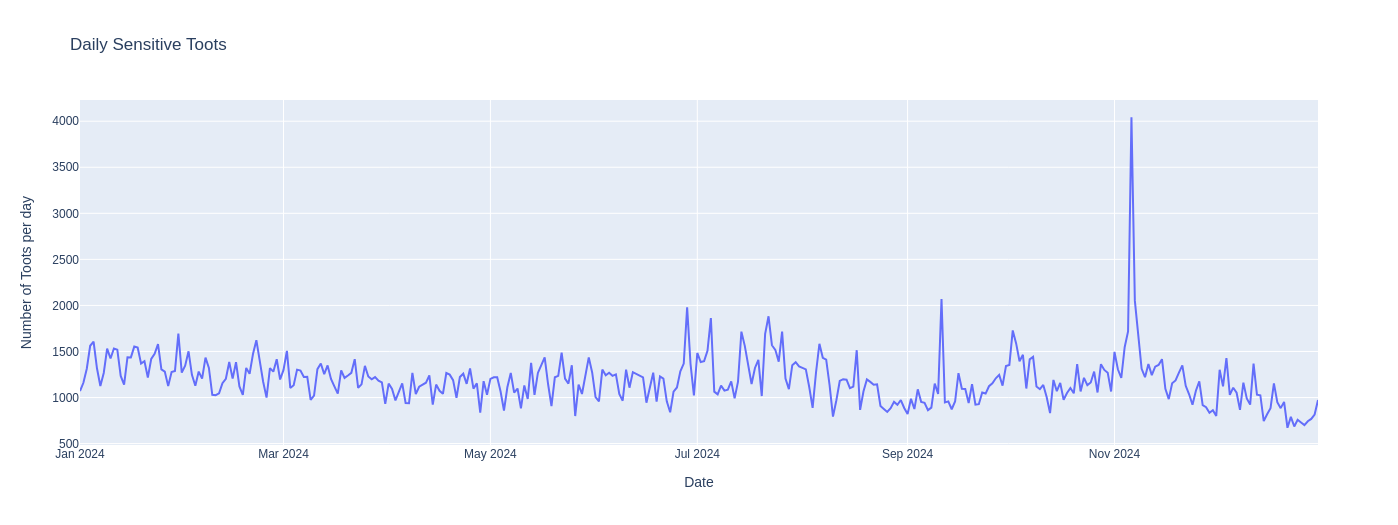
\includegraphics[width=\textwidth]{../material/sensitive_toots.png}
    \caption{Number of toots marked as sensitive in our subset per day.}
    \label{sensitive-toots}
\end{figure}